%
% 98-127
% Lecture 03: Wrangling Unity
% 
% Template adapted from
% https://www.cs.cmu.edu/~15150/previous-semesters/2012-spring/resources/latex/template.tex
%

\documentclass[11pt]{article}

\usepackage{amsmath}
\usepackage{amssymb}
\usepackage{amsthm}
\usepackage{hyperref}
\usepackage{fancyhdr}
\usepackage{listings}
\usepackage{color}
\usepackage{graphicx}
\usepackage{setspace}
\usepackage{times}
\usepackage{wrapfig}
\usepackage{fontawesome}

\usepackage{menukeys}

\oddsidemargin0cm
\topmargin-2cm
\textwidth16.5cm
\textheight23.5cm

\newtheorem{lemma}{Lemma}

%% Begin Constants %% <-- (edit these!)

% Lecture Info
\newcommand{\lecturenum}{6}
\newcommand{\lecturename}{3D Modeling in Blender}

% Author of THIS document
\newcommand{\authorname}{Adrian Biagioli}

% Course Info
\newcommand{\coursenum}{98-127}
\newcommand{\coursename}{Game Creation for People Who Want to Make Games}
\newcommand{\coursesem}{S19}

% Instructors of course
\newcommand{\instructors}{Adrian Biagioli (\,\href{mailto:abiagiol@andrew.cmu.edu}{abiagiol@andrew.cmu.edu}\,) \\ Carter Williams (\,\href{mailto:ncwillia@andrew.cmu.edu}{ncwillia@andrew.cmu.edu}\,)}

% Math shortcuts
\newcommand{\work}{\mathcal{W}}
\newcommand{\expv}{\mathbf{E}}
\newcommand{\pr}{\mathbf{Pr}}
\newcommand{\ts}{\textsuperscript}
\newcommand{\bigo}{\mathit{O}}

%% End Constants %%

%% Begin syntax highlighting settings %%

\definecolor{dkgreen}{rgb}{0,0.6,0}
\definecolor{gray}{rgb}{0.5,0.5,0.5}
\definecolor{mauve}{rgb}{0.58,0,0.82}

\lstset{frame=tb,
    language={[Sharp]C},
    aboveskip=3mm,
    belowskip=3mm,
    showstringspaces=false,
    columns=flexible,
    basicstyle={\small\ttfamily},
    numbers=left,
    stepnumber=1,
    numberstyle=\tiny\color{gray},
    keywordstyle=\color{blue},
    commentstyle=\color{dkgreen},
    stringstyle=\color{mauve},
    breaklines=true,
    breakatwhitespace=true,
    tabsize=3
  }

\lstnewenvironment{csharp}[1][]
{
  \lstset{frame=tb,
    language={[Sharp]C},
    aboveskip=3mm,
    belowskip=3mm,
    showstringspaces=false,
    columns=flexible,
    basicstyle={\small\ttfamily},
    numbers=left,
    stepnumber=1,
    numberstyle=\tiny\color{gray},
    keywordstyle=\color{blue},
    commentstyle=\color{dkgreen},
    stringstyle=\color{mauve},
    breaklines=true,
    breakatwhitespace=true,
    tabsize=3
  }
}{}

\lstnewenvironment{pseudocode}[1][]
{
    \lstset{
        mathescape=true,
        frame=tb,
        numbers=left, 
        basicstyle=\small, 
        numberstyle=\tiny\color{gray},
        keywordstyle=\color{black}\bfseries\em,
        commentstyle=\color{dkgreen},
        stringstyle=\color{mauve},
        keywords={,input, output, return, datatype, function, in, if, else, foreach, while, begin, end, }
        numbers=left,
        breaklines=true,
        breakatwhitespace=true,
        tabsize=3
    }
}
{}

% From https://tex.stackexchange.com/questions/95036/continue-line-numbers-in-listings-package
\def\ContinueLineNumber{\lstset{firstnumber=last}}
\def\StartLineAt#1{\lstset{firstnumber=#1}}
\let\numberLineAt\StartLineAt

%% End syntax highlighting settings %%

\setlength{\parindent}{2em}
\setlength{\parskip}{5pt plus 1pt}
\renewcommand{\baselinestretch}{1.15}

\pagestyle{fancyplain}
{
    \lhead{\fancyplain{}{Lecture \lecturenum}}
    \rhead{\fancyplain{}{\coursenum}}
    \chead{\fancyplain{}{\lecturename}}
}
\setlength{\headheight}{14pt}

\graphicspath{ {./images/} }

\begin{document}

\thispagestyle{plain}
{
    \vspace{1.5em}
    \begin{center}
    {
        \huge
        Lecture \lecturenum \\
        \vspace{0.5em}
        \lecturename
        \vspace{0.4em}
    } \\
    {
        \it
        \coursenum: \coursename\ \ (\coursesem)
    } \\
    \vspace{1.0em}
    Written by \authorname \\
    \vspace{0.7em}
    Instructors:\\ \instructors
    \end{center}
}

\section{Objectives}

By the end of this lesson you will be able to:
\begin{itemize}
    \item Understand the basics of the Blender user interface
    \item Build 3D models using local mesh editing tools
    \item Utilize global mesh editing tools (Modifiers)
    \item Map a texture to a 3D model using UV unwrapping
    \item Export 3D models in a Unity-optimized format
\end{itemize}

\noindent These lecture notes were written for {\bf Blender 2.79b}.  Keep in mind that at the time 
of writing, a new version with a vastly different user interface, Blender 2.8, is in beta. If you're
reading this after 2.8 is officially released, you can still enable a mode that uses keybindings
from earlier versions of Blender.  More info \href{https://wiki.blender.org/wiki/Reference/Release_Notes/2.80/UI}{here}.

We will also be looking at blender with a comparative eye towards Unity.  It may be helpful to have
some background on using Unity before looking at these notes.  Check out the Intro to Unity notes
\href{http://stage.gamecreation.org/StuCo/lectures/lec02.pdf}{here}.

\section{Downloading Blender}

\textbf{Blender} is a free and open source 3D modeling package that can be used to build assets for
your games.  You can download blender at \href{https://blender.org}{blender.org} -- make sure to
download version {\bf 2.79} for compatibility with these lecture notes.  The primary alternative to
blender, and a common option in industry, is \textbf{Autodesk Maya}.  However Maya is very expensive
for commercial use, so we will not use it in this class.  For all but the most advanced tasks,
blender has feature parity with Maya, however you may need to use Maya if you get a job at a studio.
That being said, the techniques you learn here are transferable to Maya; you'll just need to learn
the new interface.  You can download the Maya student edition (note: the student edition can not be used
for any games that you plan to sell) \href{https://www.autodesk.com/education/free-software/maya}{here}.
You are going to want to \underline{use a mouse} for this tutorial, as a mouse makes navigating 
blender's complex interface much easier.

\section{Blender Interface Basics}

{
\centering \noindent
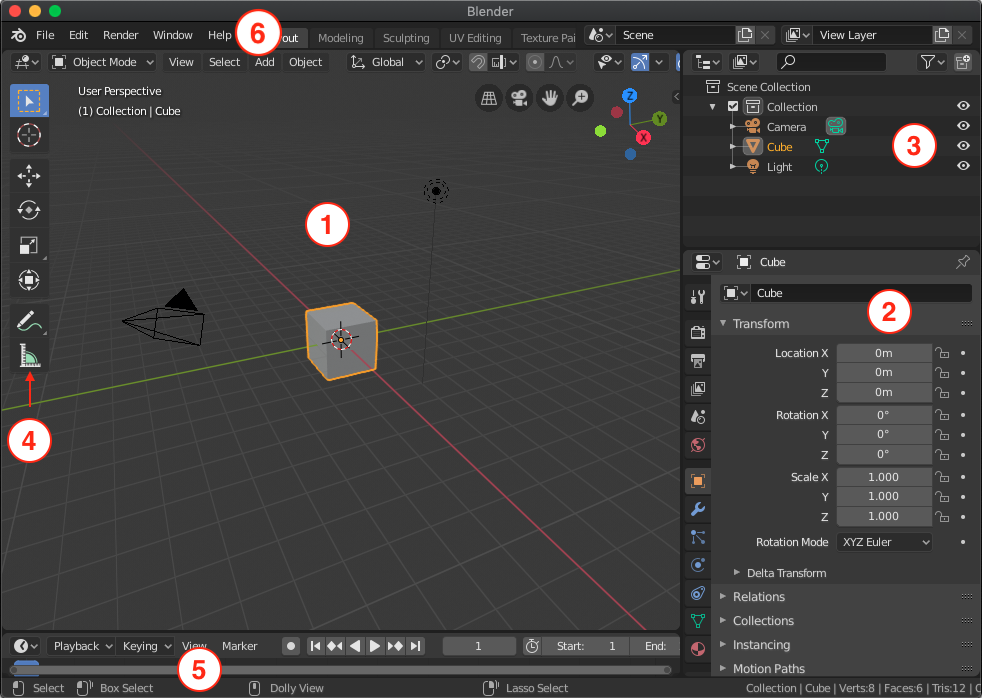
\includegraphics[width=1.0\textwidth]{blender-interface}
}

\noindent This is the default configuration of Blender when you open it for the first time.  Each
panel that you see in the above screenshot is labeled as follows:
\begin{enumerate}
    \item The \textbf{3D View} is your main view into the scene you are editing.  Unsurprisingly,
    this is where most of your work happens.  We will talk more about how to navigate the 3D view
    in the subsection below.  This is similar to the scene view in Unity.
    \item The \textbf{Properties} panel allows you to edit various properties of your scene, 
    including the camera, the currently selected object, the currently selected mesh, textures,
    materials, and so on.  We will often use the Properties panel throughout this tutorial.
    The Properties are analogous to Unity's inspector.
    \item The \textbf{Outliner} lists all of the objects, meshes, armatures (we'll get to this in a
    later lecture), and so on in your scene.  The outliner is most similar to the hierarchy view in
    Unity.
    \item The \textbf{Tool Shelf} contains shortcuts for common editing operations.  You can toggle
    the tool shelf on and off with \keys{T}.  If you ever forget a shortcut, the tool shelf is your
    friend!
    \item The \textbf{Timeline} is used to scrub through animations (we will talk about 3D animation
    in a later lecture).
    \item The \textbf{Info} panel contains common menus like \menu{File} and \menu{Window}, and
    allows you to change between preset layouts.  If you ever want to reset the blender UI, use the
    dropdown: 
\includegraphics[height=1.0em]{layout-default} and select ``Default''.

\end{enumerate}

\begin{wrapfigure}{r}[30pt]{0.17\textwidth}
    \vspace*{-2em}
    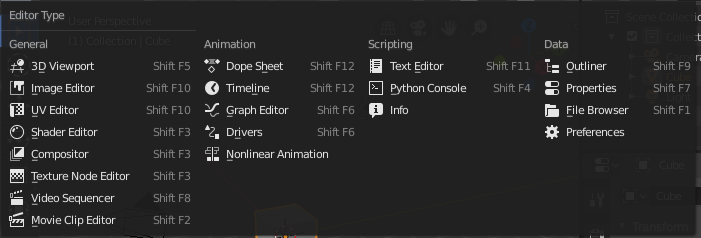
\includegraphics[width=0.17\textwidth]{editor-type-dropdown}
\end{wrapfigure}
You may have noticed that at the corner of each panel there is a dropdown.  This dropdown allows
you to change the \textit{Editor Type} of each panel.  For example, we can change from the 3D view 
to the text editor by clicking on the dropdown on the bottom left of the 3D view and selecting ``Text 
Editor.''  Fun fact: the entire blender front-end is written in python and is fully scriptable and
extendable.  The text editor is used to write python scripts for blender -- but we won't be using it
now.  Switch back to the ``3D View'' using the same dropdown.  Also notice how all of the panels
discussed on the last page are available here.  For example, it may not be all that useful, but you 
can change the 3D view into a huge timeline.

You can resize each panel by clicking and dragging at the borders.  If you want to create more editor
views than the default, \textbf{right click} on the border of two panels and select \menu{Split Area}.
Then move your mouse over the panel you would like to split and \textbf{left click} to apply.  This
process is detailed below:

{
\centering
\begin{minipage}{0.15\textwidth}
    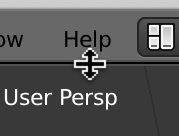
\includegraphics[width=1.0\textwidth]{split-1}\\
    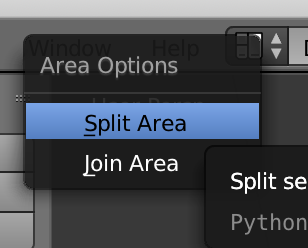
\includegraphics[width=1.0\textwidth]{split-2}
\end{minipage} $\rightarrow$
\raisebox{-.45\height}{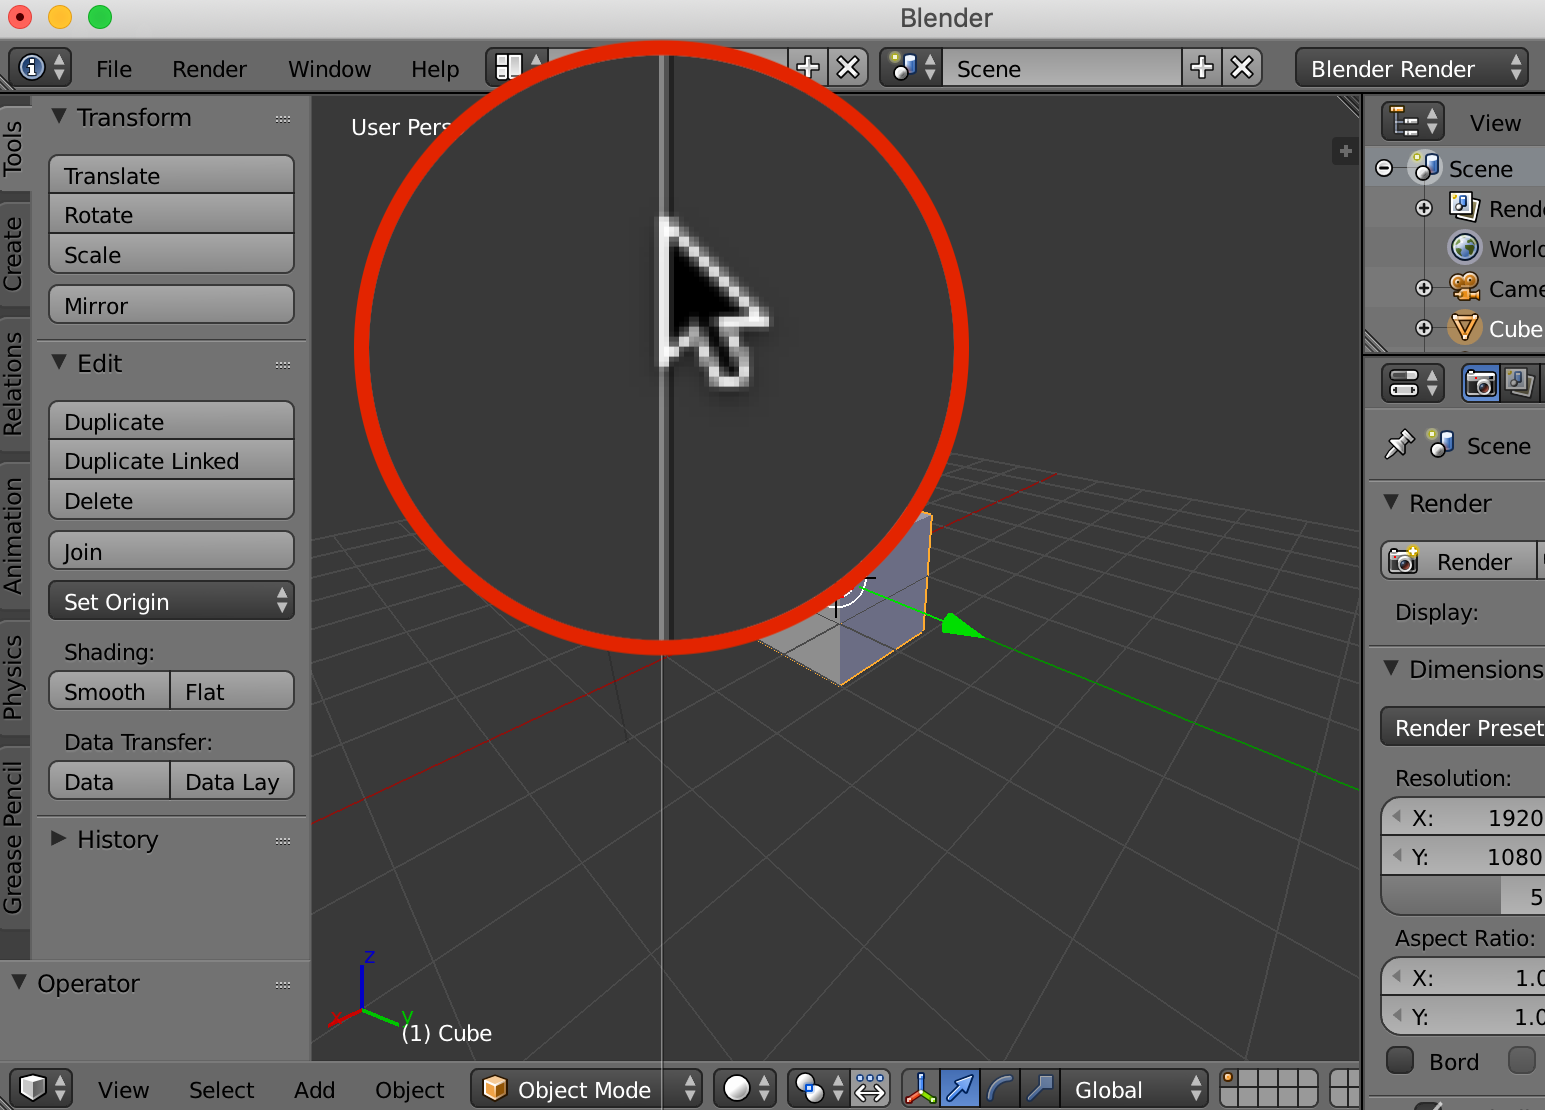
\includegraphics[width=0.36\textwidth]{split-3}} $\rightarrow$
\raisebox{-.45\height}{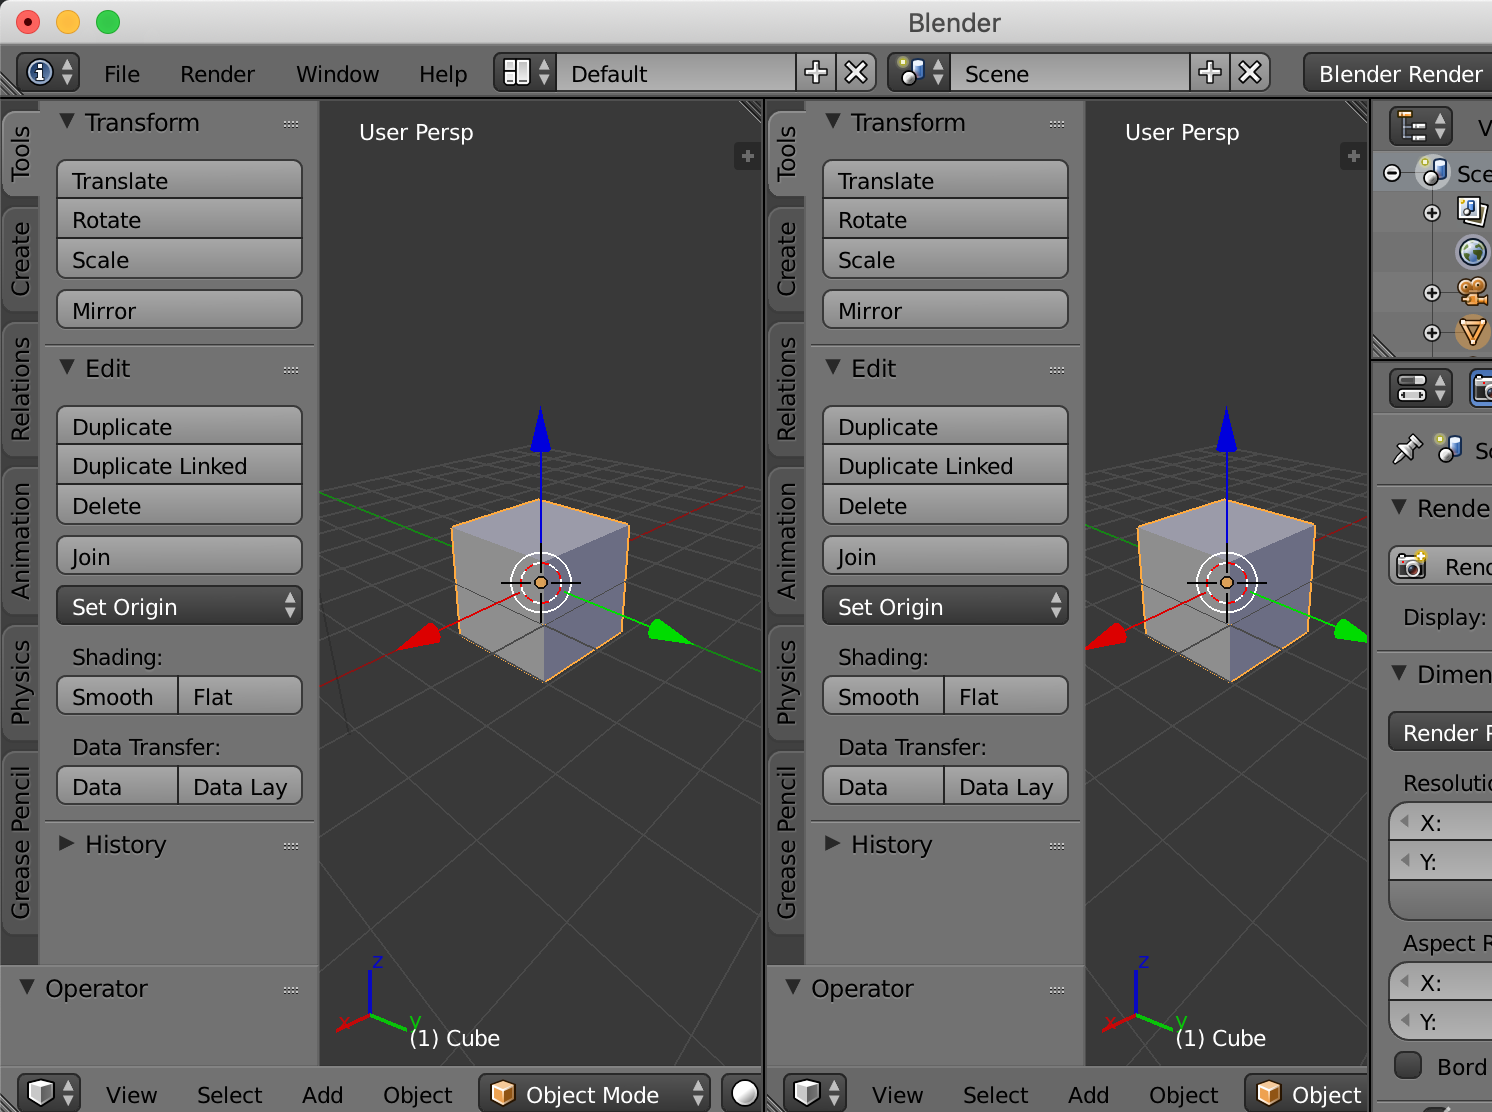
\includegraphics[width=0.36\textwidth]{split-4}}
\vspace{0.7em}
}

\noindent You can also select ``Join Area'' and click on one of the two bordering panels to join
them together.

\subsection{Navigating the 3D View}

You can navigate the 3D view using the following controls:
\begin{itemize}
    \item To \textbf{orbit} (rotate) the view, hold \keys{Middle Mouse Button} while dragging the
    mouse.
    \item To \textbf{pan} (translate) the view, hold \keys{Shift+Middle Mouse Button} while dragging
    the mouse.  You can also hold \keys{Shift+Ctrl+Midle Mouse Button} to ``Dolly Zoom'', which
    moves the camera forward and backwards.
    \item To \textbf{zoom} the view, hold \keys{Ctrl+Middle Mouse Button} while dragging the mouse,
    or scroll \keys{Mouse Wheel}.  This is different than the dolly zoom because the viewport camera
    does not move.
    \item If you ever get lost, press \keys{Numpad {\Large.}} (period) to zoom and pan to the 
    currently selected object.
\end{itemize}

\subsection{Working in Object Mode}

\begin{wrapfigure}[4]{r}[30pt]{0.3\textwidth}
    \centering \vspace*{-3.5em}
    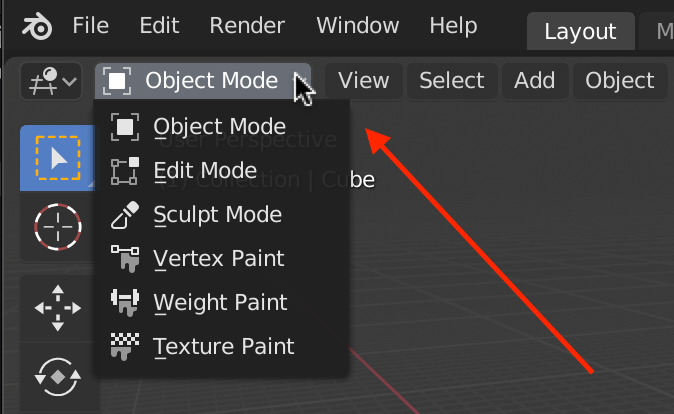
\includegraphics[width=0.3\textwidth]{mode-switcher}
    The Mode Switcher
\end{wrapfigure}
By default, when blender opens you will be in \textbf{Object Mode}.  You can verify what mode you 
are in by checking the \textit{Mode Switcher} at the bottom of the 3D View.  Each \textbf{Object} in blender
(analogous to a GameObject in Unity terminology) has a \textbf{Mesh} attached.  Just like in Unity,
you can transform Objects.  Below are some common shortcuts to manipulate objects in Object Mode 
(\textit{Important: Make sure your mouse is on top of the 3D view when using these shortcuts, because
shortcuts are different depending on which view is ``active.''})

\begin{itemize}
    \item Press \keys{Right Mouse Button} to select an object.  \textbf{Important: Left Mouse button
    does not select objects in blender!}  This is a common point of confusion for new users.
    \footnote{I know this is really confusing,  but there is hope: in the Blender 2.8 beta, the 
    developers have changed the default to left-click select.  As you can imagine, this has been a
    source of debate and nerd wars in the blender community for \textit{decades}!}
    \item Press \keys{Left Mouse Button} to move the \textit{3D cursor}.  The 3D cursor is used for
    many 3D operations as a reference point -- for now, though, you can largely ignore it.
    \item Press \keys{G} (``Grab'') to Move an object, \keys{R} (``Rotate'') to Rotate an object,
    or \keys{S} (``Scale'') to Scale an object.  You can move the mouse to control the 
    transformation; click \keys{Left Mouse Button} or press \keys{\return} to apply.  While grabbing
    / rotating / scaling, you can press \keys{X} / \keys{Y} / \keys{Z} to constrain the 
    transformation to a single axis.  Press the same key again to switch from Global axes (relative
    to the origin) to Local axes (relative to how that object is rotated).
    \item Press \keys{X} to delete an object.
    \item Press \keys{Shift+D} to duplicate an object.  You can also press \keys{Alt+D} to 
    ``Duplicate Linked,'' which shares the same mesh between the two objects.  This is similar to
    the idea of prefabs in Unity: editing the mesh of either object will affect the appearance of
    both.  This is especially useful because this link will actually persist when you import to
    Unity -- cool!
    \item Press \keys{T} to toggle on and off the Toolshelf.  The toolshelf has clickable buttons
    for many common editing operations (including all of the shortcuts listed above).
    \item Press \keys{N} to toggle on and off the \textbf{Properties} panel.  The properties panel
    allows you to directly manipulate the position / rotation / scale of whatever you have selected,
    as well as various miscellaneous settings for how the mesh displays in the 3D View.
    \item Press \keys{A} to select all or deselect all (depending on if anything is selected).
\end{itemize}

Blender has an incredibly robust shortcut system -- almost \textit{every} common editing operation
has a corresponding shortcut.  So while it may be difficult to get used to blender's UI, mastery of
it will allow you to do things very quickly.  For example, rotating an object 45 degrees in
the Z axis is as easy as \\\keys{R} \faAngleRight\ \keys{Z} \faAngleRight\ \keys{4} \faAngleRight\ 
\keys{5} \faAngleRight\ \keys{\return}.  That being said, it is still very easy to forget all of the random 
incantations--er--key combinations you need to use to do what you want.  Luckily, pressing \keys{Space} at
any time will bring up a search bar that allows you to search for any operation.  It will also show any
relevant key combinations.  You can then hit \keys{\return} to apply the operation.

\begin{center}
    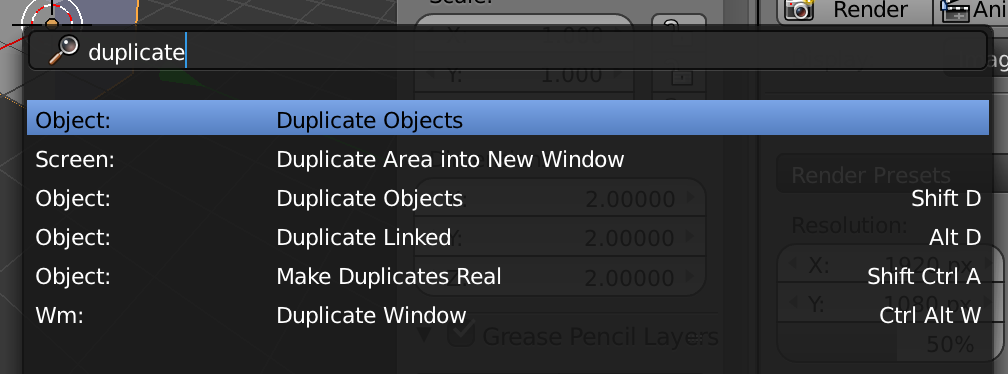
\includegraphics[width=0.5\textwidth]{search-diag}\\
    Searching for Shortcuts
\end{center}

\section{Local Mesh Editing}

\section{Using Modifiers for Global Editing Operations}

\section{Texture Mapping}

\section{Exporting to Unity}

\section{Exercise}


\end{document}